\chapter{Vecteurs Aléatoires}

Un \textbf{vecteur aléatoire} $X$ de dimension $m$ est un vecteur $X = (X_1, X_2, \dots, X_m)^T$ (souvent représenté comme un vecteur colonne) où chaque composante $X_i$ est une variable aléatoire réelle définie sur le même espace probabilisé $(\Omega, \mathcal{A}, P)$. On a déjà étudié le cas $m = 2$ avec le couple $(X, Y)$. La plupart des concepts se généralisent.

\section{Fonction de répartition d'un vecteur aléatoire}

La fonction de répartition (jointe) du vecteur aléatoire $X = (X_1, \dots, X_m)$ est la fonction $F_X : \mathbb{R}^m \to [0, 1]$ définie par :
\[
F_X(x_1, \dots, x_m) = P(X_1 \le x_1, X_2 \le x_2, \dots, X_m \le x_m)
\]
pour tous $(x_1, \dots, x_m) \in \mathbb{R}^m$.

\begin{center}
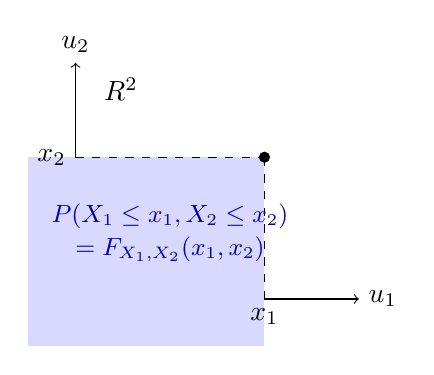
\begin{tikzpicture}[scale=1.2]
    % Axes
    \draw[->] (-0.5,0) -- (3,0) node[right] {$u_1$};
    \draw[->] (0,-0.5) -- (0,2.5) node[above] {$u_2$};
    
    % Zone bleue (Fonction de répartition)
    \fill[blue!15] (-0.5,-0.5) rectangle (2,1.5);
    
    % Lignes pointillées
    \draw[dashed] (2,0) node[below] {$x_1$} -- (2,1.5);
    \draw[dashed] (0,1.5) node[left] {$x_2$} -- (2,1.5);
    
    % Point
    \filldraw (2,1.5) circle (1.5pt);
    \node[above right] at (0.2,2) {$\mathbb{R}^2$};
    
    % Label de probabilité
    \node[align=center, blue!70!black] at (1,0.7) {\small $P(X_1 \le x_1, X_2 \le x_2)$ \\ \small $= F_{X_1,X_2}(x_1, x_2)$};
\end{tikzpicture}
\\[0.5em]
\textsc{Figure 21} – Illustration de la fonction de répartition jointe $F_{X_1,X_2}(x_1, x_2)$ pour $m=2$
\end{center}

\section{Indépendance mutuelle des composantes}

Les variables aléatoires $X_1, \dots, X_m$ sont dites \textbf{mutuellement indépendantes} si, pour tous choix d'ensembles boréliens $A_1, \dots, A_m \subset \mathbb{R}$ :
\[
P(X_1 \in A_1, X_2 \in A_2, \dots, X_m \in A_m) = P(X_1 \in A_1)P(X_2 \in A_2) \dots P(X_m \in A_m)
\]
Cela est équivalent à dire que la fonction de répartition jointe est le produit des fonctions de répartition marginales :
\[
F_X(x_1, \dots, x_m) = F_{X_1}(x_1)F_{X_2}(x_2) \dots F_{X_m}(x_m) \quad \text{pour tous } (x_1, \dots, x_m)
\]
Si les $X_i$ admettent des densités marginales $f_{X_i}$, alors l'indépendance mutuelle est équivalente à ce que la densité jointe du vecteur $X$ soit le produit des densités marginales : $f_X(x_1, \dots, x_m) = f_{X_1}(x_1)f_{X_2}(x_2) \dots f_{X_m}(x_m)$ (presque partout).
\subsection{Espérance d'un vecteur aléatoire}

L'espérance du vecteur aléatoire $X = (X_1, \dots, X_m)^T$ est le vecteur (colonne) des espérances de ses composantes (si elles existent) :
\[
\E[X] = \begin{pmatrix} 
\E[X_1] \\ \E[X_2] \\ \vdots \\ \E[X_m] 
\end{pmatrix} = (\E[X_1], \E[X_2], \dots, \E[X_m])^T
\]

\subsection{Matrice de Covariance}

La \textbf{matrice de covariance} du vecteur aléatoire $X = (X_1, \dots, X_m)^T$ est une matrice carrée de taille $m \times m$, notée $\Cov(X)$ ou $\Sigma$, dont l'élément $(i, j)$ est $\Sigma_{ij} = \Cov(X_i, X_j)$.

\[
\Sigma = \begin{pmatrix}
\Var(X_1) & \Cov(X_1, X_2) & \dots & \Cov(X_1, X_m) \\
\Cov(X_2, X_1) & \Var(X_2) & \dots & \Cov(X_2, X_m) \\
\vdots & \vdots & \ddots & \vdots \\
\Cov(X_m, X_1) & \Cov(X_m, X_2) & \dots & \Var(X_m)
\end{pmatrix}
\]

Notez que $\Cov(X_i, X_i) = \Var(X_i)$. La matrice de covariance peut aussi s'écrire de manière compacte en utilisant les vecteurs d'espérance $\mu = \E[X]$ :
\[
\Sigma = \E[(X - \mu)(X - \mu)^T]
\]
où $(X - \mu)$ est un vecteur colonne et $(X - \mu)^T$ est son transposé (vecteur ligne), leur produit est donc une matrice $m \times m$. Propriétés de la matrice de covariance :
\begin{itemize}
    \item $\Sigma$ est \textbf{symétrique} : $\Sigma_{ij} = \Cov(X_i, X_j) = \Cov(X_j, X_i) = \Sigma_{ji}$.
    \item $\Sigma$ est \textbf{semi-définie positive} : pour tout vecteur constant non nul $\mathbf{a} \in \mathbb{R}^m$, $\mathbf{a}^T \Sigma \mathbf{a} = \Var(\mathbf{a}^T X) \ge 0$.
    \item Si les composantes $X_i$ sont \textbf{mutuellement indépendantes} (ou simplement non corrélées deux à deux), alors $\Cov(X_i, X_j) = 0$ pour $i \neq j$. Dans ce cas, $\Sigma$ est une \textbf{matrice diagonale} avec les variances $\Var(X_i)$ sur la diagonale.
\end{itemize}

\subsection{Distribution Multinomiale}

La loi multinomiale est une généralisation de la loi binomiale à des expériences ayant plus de deux issues possibles.

\begin{definition}[Loi Multinomiale]
Considérons une expérience aléatoire qui peut avoir $k$ issues (ou catégories) possibles, mutuellement exclusives, $R_1, R_2, \dots, R_k$. Supposons que la probabilité de l'issue $R_j$ est $p_j$, avec $p_j \ge 0$ pour tout $j = 1, \dots, k$ et $\sum_{j=1}^k p_j = 1$. On répète cette expérience $n$ fois de manière indépendante. Soit $X_j$ le nombre de fois que l'issue $R_j$ est observée au cours des $n$ répétitions. Le vecteur aléatoire $X = (X_1, X_2, \dots, X_k)$ suit une \textbf{loi multinomiale} de paramètres $n$ (nombre d'essais) et $(p_1, p_2, \dots, p_k)$ (probabilités des issues), notée $X \sim \mathcal{M}(n; p_1, \dots, p_k)$.
\end{definition}
\begin{center}
\renewcommand{\arraystretch}{1.5}
$\begin{pmatrix}
\colorbox{diagblue}{$\Var(X_1)$} & \colorbox{covgreen}{$\Cov(X_1, X_2)$} & \colorbox{covgreen}{$\Cov(X_1, X_3)$} \\
\colorbox{covgreen}{$\Cov(X_2, X_1)$} & \colorbox{diagblue}{$\Var(X_2)$} & \colorbox{covgreen}{$\Cov(X_2, X_3)$} \\
\colorbox{covgreen}{$\Cov(X_3, X_1)$} & \colorbox{covgreen}{$\Cov(X_3, X_2)$} & \colorbox{diagblue}{$\Var(X_3)$}
\end{pmatrix}$

\vspace{0.5em}
\small
Structure de la matrice de covariance $\Sigma$ pour $m = 3$. \\
Les termes sur la diagonale (bleu) sont les variances. \\
Les termes hors diagonale (vert) sont les covariances. \\
La matrice est symétrique ($\Cov(X_i, X_j) = \Cov(X_j, X_i)$).

\vspace{0.5em}
\textsc{Figure 22} – Illustration de la Matrice de Covariance $\Sigma$ pour un vecteur aléatoire $(X_1, X_2, X_3)^T$.
\end{center}

\vspace{1em}

Notez que les $X_j$ ne sont pas indépendantes car leur somme est fixée : $\sum_{j=1}^k X_j = n$. La fonction de masse conjointe du vecteur $X$ est :
\[
P(X_1 = n_1, X_2 = n_2, \dots, X_k = n_k) = \frac{n!}{n_1! n_2! \dots n_k!} p_1^{n_1} p_2^{n_2} \dots p_k^{n_k}
\]
pour tous entiers $n_j \ge 0$ tels que $\sum_{j=1}^k n_j = n$. Si cette condition n'est pas remplie, la probabilité est nulle. Le terme $\frac{n!}{n_1! n_2! \dots n_k!}$ est le \textbf{coefficient multinomial}, noté $\binom{n}{n_1, n_2, \dots, n_k}$.

\paragraph{Propriétés de la loi multinomiale :}
\begin{itemize}
    \item Chaque composante $X_j$ (prise isolément) suit une loi binomiale $\mathcal{B}(n, p_j)$.
    \item Espérance : $\mathbb{E}[X_j] = np_j$.
    \item Variance : $\text{Var}(X_j) = np_j(1 - p_j)$.
    \item Covariance : Pour $i \neq j$, $\text{Cov}(X_i, X_j) = -np_i p_j$. (La covariance négative reflète le fait que si une issue se produit plus souvent, les autres doivent se produire moins souvent, puisque la somme des occurrences est fixée à $n$).
\end{itemize}

\paragraph{Origine de la formule de la loi multinomiale} La probabilité $P(X_1 = n_1, \dots, X_k = n_k)$ est le produit de deux termes :
\begin{enumerate}
    \item \textbf{Le nombre de façons de choisir les positions pour chaque résultat :} Il y a $n$ répétitions de l'expérience. On doit choisir $n_1$ positions (essais) où l'issue $R_1$ se produit, puis $n_2$ positions parmi les $n - n_1$ restantes pour $R_2$, et ainsi de suite. Le nombre de façons de partitionner les $n$ essais en $k$ groupes de tailles $n_1, n_2, \dots, n_k$ est donné par le coefficient multinomial :
    \[ \binom{n}{n_1, n_2, \dots, n_k} = \frac{n!}{n_1! n_2! \dots n_k!} \]
    \item \textbf{La probabilité d'une séquence spécifique d'observations :} Considérons une séquence particulière d'observations où $R_1$ apparaît $n_1$ fois, $R_2$ apparaît $n_2$ fois, etc. En raison de l'indépendance des $n$ répétitions, la probabilité d'une telle séquence spécifique est $p_1^{n_1} p_2^{n_2} \dots p_k^{n_k}$.
\end{enumerate}

\vspace{1em}
La probabilité totale est le produit du nombre de ces séquences par la probabilité de n'importe laquelle d'entre elles (puisqu'elles sont toutes équiprobables).

\section{ Distributions Conditionnelles}

Soient $X$ et $Y$ deux variables aléatoires définies sur le même espace probabilisé. On s'intéresse à la loi de $X$ sachant que $Y$ a pris une certaine valeur $y$. C'est la "loi de $X$ conditionnellement à $Y=y$".

\paragraph{Cas où $X, Y$ sont discrètes :} Si $P(Y=y_j) > 0$, la \textbf{fonction de masse conditionnelle} de $X$ sachant $Y=y_j$ est :

$$P(X=x_i | Y=y_j) = \frac{P(X=x_i, Y=y_j)}{P(Y=y_j)}$$

Pour un $y_j$ fixé, $P(X=x_i | Y=y_j)$ est une fonction de masse en $x_i$ (sa somme sur toutes les valeurs $x_i$ possibles vaut 1). L'\textbf{espérance conditionnelle} de $g(X)$ sachant $Y=y_j$ est :

$$E[g(X) | Y=y_j] = \sum_{i} g(x_i) P(X=x_i | Y=y_j)$$

\paragraph{Cas où $X, Y$ sont conjointement continues :} Si $(X, Y)$ a une densité jointe $f_{X,Y}(x,y)$ et si la densité marginale $f_Y(y) > 0$. La \textbf{densité conditionnelle} de $X$ sachant $Y=y$ est définie par :

$$f_{X|Y=y}(x) = \frac{f_{X,Y}(x,y)}{f_Y(y)}$$

Pour un $y$ fixé, $f_{X|Y=y}(x)$ est une fonction de $x$ et c'est une densité de probabilité (positive et d'intégrale 1 sur $\mathbb{R}$). L'\textbf{espérance conditionnelle} de $g(X)$ sachant $Y=y$ est :

$$E[g(X) | Y=y] = \int_{-\infty}^{+\infty} g(x) f_{X|Y=y}(x) \, dx$$

\vspace{1em}

\begin{exemple}[Illustration des distributions conditionnelles lancers de pièce.] 
    Soit $X = \text{gain total}$ (Pile $= +1$~euro, Face $= 0$~euro), $X \in \{0, 1, 2, 3\}$. Soit $Y = \text{résultat du 1er lancer}$ (1 si Pile, 0 si Face), $Y \in \{0, 1\}$. Supposons les lancers indépendants et les pièces équilibrées. La loi jointe $P(X=x, Y=y)$ (en 8èmes) a été établie précédemment (voir tableau Section 3.2 - implicitement, car les calculs y mènent). La loi marginale de $Y$ est $P(Y=0) = 4/8 = 1/2$ et $P(Y=1) = 4/8 = 1/2$. La loi de $X$ conditionnellement à $Y=0$ (notée $X|_{Y=0}$) est donnée par $P(X=x \mid Y=0) = \frac{P(X=x, Y=0)}{P(Y=0)}$ : $P(X=0 \mid Y=0) = \frac{P(X=0, Y=0)}{1/2}$. Par exemple, si les 3 lancers donnent FFF, $(X=0, Y=0)$ a proba $1/8$. Donc $P(X=0 \mid Y=0) = (1/8)/(1/2) = 1/4$. De même, $P(X=1 \mid Y=0) = \frac{P(X=1, Y=0)}{1/2}$. L'événement $(X=1, Y=0)$ correspond à (F,P,F) ou (F,F,P), proba $2/8$. Donc $P(X=1 \mid Y=0) = (2/8)/(1/2) = 1/2$. $P(X=2 \mid Y=0) = \frac{P(X=2, Y=0)}{1/2}$. L'événement $(X=2, Y=0)$ correspond à (F,P,P), proba $1/8$. Donc $P(X=2 \mid Y=0) = (1/8)/(1/2) = 1/4$. $P(X=3 \mid Y=0) = 0$. (Intuitivement, si le premier lancer est Face ($Y=0$), le gain $X$ est le nombre de Piles sur les 2 lancers suivants, donc $X|_{Y=0} \sim \mathcal{B}(2, 1/2)$.) De même pour $X|_{Y=1}$ : $P(X=1 \mid Y=1) = 1/4$, $P(X=2 \mid Y=1) = 1/2$, $P(X=3 \mid Y=1) = 1/4$.
\end{exemple}

\noindent \textbf{Expérience aléatoire avec une probabilité de succès $p$ inconnue (Introduction à l'Inférence Bayésienne)} \quad On s'intéresse à un paramètre inconnu $p$ (par exemple, la probabilité de succès d'une expérience de Bernoulli). Dans l'approche bayésienne, on traite $p$ comme une variable aléatoire, dotée d'une distribution a priori (reflétant notre croyance sur $p$ avant toute observation). Supposons un a priori uniforme pour $p$ sur $[0, 1] : p \sim \mathcal{U}([0, 1])$, donc sa densité $f_P(p) = 1$ pour $p \in [0, 1]$. On réalise ensuite $N_{tot} = n+m$ fois l'expérience et on observe $n$ succès et $m$ échecs. On souhaite mettre à jour notre croyance sur $p$ en calculant sa distribution a posteriori, conditionnellement aux données observées. La vraisemblance d'observer $n$ succès et $m$ échecs, si la probabilité de succès est $p$, est donnée par la loi binomiale : $L(\text{données}|p) = \binom{n+m}{n} p^n (1-p)^m$. Par le théorème de Bayes (version continue pour les densités) : $f_{P|\text{données}}(p|\text{données}) \propto L(\text{données}|p) f_P(p)$. $f_{P|\text{données}}(p|n \text{ succès}, m \text{ échecs}) \propto p^n (1-p)^m \cdot 1$ (pour $p \in [0, 1]$). La densité a posteriori est donc de la forme $C \cdot p^n (1-p)^m$. C'est la densité d'une loi Beta, plus précisément $\mathcal{B}eta(n+1, m+1)$. La constante $C$ est la constante de normalisation $1/B(n+1, m+1)$, où $B$ est la fonction Beta.

\subsection*{4.7 \quad Espérance Conditionnelle comme Variable Aléatoire}

Jusqu'à présent, $\mathbb{E}[X|Y=y]$ était un nombre (ou une fonction de la valeur $y$). On peut définir $\mathbb{E}[X|Y]$ comme une \textbf{variable aléatoire}. C'est une fonction de la variable aléatoire $Y$, et donc elle-même une variable aléatoire. On la note souvent $h(Y)$, où la fonction $h$ est définie par $h(y_j) = \mathbb{E}[X|Y=y_j]$ dans le cas discret (ou $h(y) = \mathbb{E}[X|Y=y]$ dans le cas continu). Cette variable aléatoire $\mathbb{E}[X|Y]$ prend la valeur $\mathbb{E}[X|Y=y]$ lorsque l'événement $\{Y=y\}$ se réalise.

\vspace{1em}

\begin{definition} [Espérance Conditionnelle. (formelle)] L'espérance conditionnelle $\mathbb{E}[X|Y]$ de $X$ sachant $Y$ est l'unique variable aléatoire $Z$ telle que :

\begin{enumerate}
    \item $Z$ est $\sigma(Y)$-mesurable (intuitivement, $Z$ est une fonction de $Y$, $Z = h(Y)$, et ne dépend que de l'information apportée par $Y$).
    \item Pour tout événement $A \in \sigma(Y)$ (c'est-à-dire, tout événement dont la réalisation ou non ne dépend que de $Y$, typiquement $A = \{Y \in B\}$ pour un borélien $B$), on a :
    $$\mathbb{E}[Z \cdot \mathbf{1}_A] = \mathbb{E}[X \cdot \mathbf{1}_A]$$
\end{enumerate}

\noindent où $\mathbf{1}_A$ est la fonction indicatrice de $A$.
\end{definition}
\vspace{1em}

Cette définition est plus abstraite et générale. Elle stipule que $\mathbb{E}[X|Y]$ est la "meilleure approximation" de $X$ en termes de variables aléatoires qui sont fonctions de $Y$ (au sens de la projection orthogonale dans l'espace $L^2$ si les variables sont de carré intégrable).

\begin{proposition}[Propriétés de l'espérance conditionnelle]
Soient $X, X_1, X_2, Y$ des variables aléatoires et $a, b \in \mathbb{R}$.
\begin{enumerate}
    \item \textbf{Linéarité :} $\E[aX_1 + bX_2|Y] = a\E[X_1|Y] + b\E[X_2|Y]$ (p.s.).
    \item \textbf{Espérance d'une constante :} Si $c$ est une constante, $\E[c|Y] = c$ (p.s.).
    \item \textbf{Sortir ce qui est $\sigma(Y)$-mesurable ("connu sachant $Y$") :} Si $g$ est une fonction mesurable telle que $g(Y)$ soit une v.a. bien définie, alors $\E[g(Y)X|Y] = g(Y)\E[X|Y]$ (p.s.). En particulier, $\E[g(Y)|Y] = g(Y)$ (p.s.).
    \item \textbf{Indépendance :} Si $X \indep Y$, alors $\E[X|Y] = \E[X]$ (p.s.). (La connaissance de $Y$ n'apporte aucune information sur $X$).
    \item \textbf{Espérance itérée (Tower property / Loi de l'espérance totale) :} 
    \[ \E[\E[X|Y]] = \E[X] \]
\end{enumerate}
C'est une propriété fondamentale et très utile pour calculer des espérances en conditionnant.
\end{proposition}

\begin{exemple}[Produit de convolution]
Si $X \indep Y$ sont deux variables aléatoires continues indépendantes, et $Z = X + Y$. On veut trouver la densité $f_Z(z)$. On peut utiliser la loi de l'espérance totale pour la fonction de répartition $F_Z(z) = P(X + Y \le z) = \E[\mathbf{1}_{X+Y \le z}]$.
$F_Z(z) = \E[\E[\mathbf{1}_{X+Y \le z}|Y]]$. L'espérance intérieure est $\E[\mathbf{1}_{X+Y \le z}|Y = y] = P(X + y \le z | Y = y) = P(X \le z - y | Y = y)$. 

Par indépendance de $X$ et $Y$, $P(X \le z - y | Y = y) = P(X \le z - y) = F_X(z - y)$. Donc, l'espérance conditionnelle $\E[\mathbf{1}_{X+Y \le z}|Y]$ est la variable aléatoire $F_X(z - Y)$.
Ainsi, $F_Z(z) = \E[F_X(z - Y)] = \int_{-\infty}^{+\infty} F_X(z - y)f_Y(y) \, dy$. Pour obtenir la densité $f_Z(z) = \frac{d}{dz}F_Z(z)$, en dérivant sous le signe intégral (sous conditions de régularité) :
\[ f_Z(z) = \int_{-\infty}^{+\infty} \left( \frac{d}{dz} F_X(z - y) \right) f_Y(y) \, dy = \int_{-\infty}^{+\infty} f_X(z - y)f_Y(y) \, dy \]
C'est la formule du \textbf{produit de convolution} des densités $f_X$ et $f_Y$, noté $(f_X * f_Y)(z)$.
\end{exemple}